
% explain that modern ISAs dont have timing semantics, that's why we provide assembly level instructions to help programmers control timing in the ISA
The Instruction-set architecture (ISA) serve as the contract between the software and the hardware.
The programmer understands the semantics of each instruction and use it to construct programs.
Computer architects ensure that the implementation of each instruction abides to the semantics specified in the ISA.
The semantics of the instructions in modern ISAs often do not specify temporal meaning to the instructions.   
Thus, in order to reason about the temporal properties of a program, we must step outside of the ISA semantics and dive deep into the architectural details.
Since ISAs do not provide any means of exposing or controlling the timing behavior of software, their implementations are under no obligations to exhibit predictable and repeatable timing behaviors.
This makes the reasoning of temporal behaviors of programs even more difficult.  
In the previous sections, we presented a predictable computer architecture that implements timing predictable behaviors for conventional instructions in the ISA. 
In this section, we will present our initial efforts to extend the ISA with timing properties.  
Our vision is to bring temporal meaning to the semantics of ISA which allows us to reason about timing of programs independent of the platform.
This allows higher-level models with temporal semantics, such as models expressed using e.g. MathWorks Simulink\textsuperscript{\textregistered} or Giotto~\cite{henzinger_giotto}, to be more easily synthesized into lower-level implementations, such as C code, without deeply coupling the design to a particular hardware platform. 

A naive way to the extend the ISA with timing properties would be to associate with each instruction a constant execution time. 
This \emph{constant time} ISA provides a clear timing definition to all programs written with it.
The semantics of the program would include the execution time of basic blocks, and any underlying architecture implementation must conform to it.
All programs written with the \emph{constant time} ISA can also be ported across different architectures of the same family and maintain the same timing behavior.
This also means that any architecture implementation that does not exhibit the defined timing properties is an incorrect implementation.
A \emph{constant time} ISA would allow the reasoning of temporal properties independent of architecture, and engrave in the semantics of programs temporal definitions.     
However, the major limitation of the \emph{constant time} ISA is that it prevents performance improvements at the micro-architectural level, as instruction execution time must conform to the constant time specified in the ISA.
Modern ISAs allow computer architects to freely innovate in architectural techniques to speed up execution time of instructions while still conforming to the semantics of the ISA.  
The program performance improves as the architecture performance improves, without any effort from the programmer. 
By associating a constant execution time for each instruction, the \emph{constant time} ISA over constrains the performance of programs, and limits the innovation of architecture implementations.    

Instead of associating with all instructions a constant execution time, we extend the ISA by adding assembly level instructions that allow us to control the timing behavior of programs. 
Ip and Edwards~\cite{ip2006processor} proposed a simple extension to the processor which implemented the \emph{deadline} instruction, an instruction that allows the programmer to specify a minimum execution time of code blocks.
They showed an implementation of a VGA controller that uses the deadline instructions to send out the horizontal and vertical sync signals in software.
We further expand on this concept of controlling execution time in software, and introduce a set of assembly timing instructions that allows us to 
control not only the minimum execution time, but also handle cases where the execution time exceeds a specified deadline.

It is currently already possible to manipulate external timers and set interrupts in most modern embedded platforms.
However, the procedure of setting timing interrupts highly varies depending on platform implementation.
Access to external timers are often done through memory mapped registers, which views the external timer as another I/O component.
As a result, the timing behavior of the program is deeply tied to the underlying implementation platform.
By defining the timing instructions as part of the instruction set, we unify the semantics of time across all programs implemented using the ISA, and any correct implementation must conform to the timing specifications in the software.
This brings the \emph{control} of timing up to software, instead of it being a side effect of the underlying architecture implementation.  
In this section, we will introduce the timing instructions added to the instruction set that allow us to experiment and investigate the effects and possibilities of extending ISA with timing properties.
Formally defining the ISA extensions is part of an ongoing work for the PRET project.
Here, we describe informally their semantics and through illustrative examples we will also present their usage. 
In section~\ref{sec:ptarm_instructions} we will present the implementation and timing details of these instructions.

\subsection{Timing Instructions}
Our extension of the ISA assumes a \emph{platform clock} that is synchronous with the execution of instructions.
This \emph{platform clock} is used by all timing instructions to specify and manipulate the execution time of code blocks.
The representation of \emph{time} in the ISA is in itself an interesting topic of research.
For example, IEEE 1588 timestamps use 32 bits of nanoseconds and 48 bits of seconds to represent time.    
Our current implementation uses 64 bits of nanoseconds in the \emph{platform clock} to represent time. 
We choose this representation for several reasons. 
First, with our timing instructions, timestamps are obtained by the programmer and can be manipulated throughout the program with data operating instructions.
Typical datapaths and registers are 32 bits. 
By using 64 bits of nanoseconds to represent time, programmers can use \emph{add with carry} instructions to manage with overflow of 64 bit additions without extra overhead. 
On the other hand, if we used the IEEE 1588 timestamp format to represent time, then any manipulation of time through the software would require explicit checking of the nanoseconds overflowing to the seconds register.
Second, the 64 bit nanoseconds simplifies the hardware implementation and comparisons of the \emph{platform clock} and timestamp values.
In chapter~\ref{chapter:ptarm} we will show our implementation, which utilizes the existing datapath and integrates the \emph{platform clock} deeply into the architecture. 

Unsigned 64 bits of nanoseconds can only represent time up to a little more than 584 years, so the \emph{platform clock} in our ISA is meant for a local representation of time. 
The \emph{platform clock} is reset to zero on processor reset. 
Even though the timing instructions operate on the exact 64 bit value of time, they are used control offsets of time. 
The actual value of the timestamp is merely used to calculate the elapsed time of code blocks.
For distributed systems that require communication of timestamps across platforms, the consistent view of time across platforms must be obtained.
This can occur during system initialization, where the global time is obtained and kept in the system.  
This initial global time can be appended to the current platform time to obtain the current global time. 
For systems designed run longer than 584 years each reset, the overflow of the 65th bit must be managed in software to ensure a consistent view of time.


\begin{table}[h]
\noindent\makebox[\textwidth]{%
\begin{smalltabular}{ | l | p{10cm} | }
  \hline                        
  Instruction & Description \\ \hline
  \textbf{\textit{get\_time}} &
\gettime\ is used to obtain the current platform time. 
  \\ \hline 
  \textbf{\textit{delay\_until}} &
\delayuntil\ is used to delay the execution of the program until a certain timestamp.   
 \\ \hline
   \textbf{\textit{exception\_on\_expired}} & 
\exceptiononexpire\ is used to register timestamps that trigger timing exceptions when the platform time exceeds the registered timestamp.  
\\ \hline
   \textbf{\textit{deactivate\_exception}} & 
\deactivateexception\ is used to deactivate the registered timestamps that trigger timing exceptions.
\\ \hline
\end{smalltabular}}
\caption{List of assembly timing instructions}
\label{table:timing_instructions}
\end{table}

Table~\ref{table:timing_instructions} shows the timing instructions and a brief description of their functionality.   
Our current implementation extends the ARM~\cite{armrefman} instruction set, so here we will present our timing instruction extensions in the context of the ARM ISA.
However, the concepts and extensions could easily be applied to other ISAs. 
The ARM ISA sets aside an instruction encoding space to allow additions to the architecture with co-processor extensions. 
Our timing instructions are currently implemented using the co-processor instruction encoding, which also enables us to use conventional ARM cross-compilers to compile programs and test our architecture.     

\subsubsection{Get\_Time}
The \gettime\ instruction is mainly used to obtain the time on the \emph{platform clock}.
This instruction interfaces the program with the current platform time by loading the 64 bit timestamp of the current platform time in general purpose registers. 
The timestamps are stored in general purpose registers to make it accessible to programmers. 
The programmer can manipulate the timestamps by using conventional data-processing instructions like add or subtract.
However, because the timestamp is 64 bits, architectures with 32 bit registers store the value in 2 separate registers. 
Thus, any manipulation of timestamps must handle the overflow  properly from 32 bits operations. 
Several ISAs provide an \emph{add with carry} instruction that can be used, or else the programmer must explicitly do so in software.
The timestamp is used as inputs to other timing instructions which we will introduce below.   

If the \emph{platform clock} was memory mapped to two 32 bit memory locations, then the functionality of this instruction could technically be implemented by the reading of memory mapped addresses. 
This would be similar to conventional methods of accessing timers. 
However, loading a 64 bit time value would possible require 2 consecutive loads.
Without care, the programmer could easily read 2 inconsistent 32 bit values of time, because the platform time continues to elapse in between the 2 reads.     
Even if a 64 bit load instruction is present in the ISA, the ISA makes no guarantee that a loaded 64 bit value from main memory would contain a consistent timestamp value from the same point in time. 
Thus, to make explicit the nature of the operation, we use a separate instruction that ensures the programmer will get a consistent 64 bit timestamp from a single point in time.    
In our implementation, this single point of time is when the \gettime\ instruction enters the pipeline.

\subsubsection{Delay\_Until}
The \delayuntil\ instruction is used to delay program execution until a specified time.
The effect is similar to the one presented by Ip and Edwards~\cite{ip2006processor}, where the programmer can specify a minimum execution time for a code block.
The difference is, in our ISA, the unit of time is represented by nanoseconds, instead of processor cycles.
The \delayuntil\ instruction takes as input a timestamp, usually derived from the timestamp obtained from \gettime, and compares it to the current platform time to determine if delays are needed.
Listing~\ref{lst:delay-until-sample} shows an example of how \delayuntil\ and \gettime\ are used together to control a minimum execution time a code block.
The assembly code is written using the ARM instruction set.
The timing instructions are implemented as co-processor 13 instructions, so all timing instructions are in the format \textbf{\textit{cdp, p13, $<$opcode$>$ rd, rn, rm, 0}}.
\Gettime\ has an opcode of 8, and \delayuntil\ has an opcode of 4.

\begin{lstlisting}[float=h, label=lst:delay-until-sample,caption=Sample assembly code of delay\_until ]
cdp p13, 8, c2, c0, c0, 0  ; {c2,c3} = platform time (get_time)
adds r3, r3, #400          ; c3 += 400 (save carry)
adc r2, r2, #0             ; c2 = c2 + <previous carry> 

add r5, r6, r6             ; code block to execution

cdp p13, 4, c2, c2, c3, 0  ; delay_until 
b end
\end{lstlisting}

In the code sample, lines 1 through 3 setup the timestamp that is passed into \delayuntil. 
\Gettime\ is used to obtain the current platform time, and an offset of 400 nanoseconds is added to the timestamp with \emph{adds} and \emph{adc} instructions.
The \emph{adds} instruction does a 32 bit add and saves the carry bit in the processor state register, so \emph{adc} can use the carry along with its 32 bit addition.
The 400 nanosecond offset added to the timestamp is the minimum execution time specified for the code between \gettime\ and \delayuntil.
This also includes time it takes to compute the deadline timestamp, as both \emph{adds} and \emph{adc} instructions execute between \gettime\ and \delayuntil.
When the \delayuntil\ instruction is decoded, the deadline timestamp is checked against platform time.
The program will be delayed until platform time passes the deadline timestamp. 
If platform time has already passed the deadline timestamp, then this \delayuntil\ instruction will simply act as a \emph{nop}, and the program will continue to execute. 

It is important to know that \delayuntil\ merely specifies a minimum execution time.
If the execution of the code block takes longer than the specified offset to execution, \delayuntil\ will have no effect on the program.
Thus, \delayuntil\ should not be used to enforce real-time constraints.
Instead, \delayuntil\ can be used to synchronize programs with external sources. 
For example, the VGA controller presented in~\cite{ip2006processor} is implemented with the same mechanics to send the horizontal and vertical sync signals to the monitor from software.
In chapter~\ref{chapter:app} we will also show applications that use this mechanism to synchronize the communication of hardware threads, and remove the execution time variance exhibited by software control paths.  
    
% \subsubsection{Delay\_and\_Set}
% The \delayandset\ instruction is an extension of the \delayuntil\ instruction with the additional ability to update the deadline timestamp with an offset. 
% This instruction has similar behavior to the \emph{deadline instruction} introduced in~\cite{ip2006processor}.
% Just as \delayuntil, \delayandset\ takes in an input timestamp and delays program execution until platform time exceeds the input timestamp. 
% However, \delayandset\ takes in an additional register, storing a 32 bit nanosecond value, used to update the input timestamp.
% Based on instruction flags, \delayandset\ can add the offset value to the current timestamp, or the current platform time after it has exceeded the timestamp value. 
% This has subtle impact on jitter and loop timing, which we will further explore in section~\ref{sec:timing_instruction_usage_notes}.  
% 
% \Delayandset\ is used when the timing constraints for control loops are tight, because it can delay the program and set the next timestamp in one instruction. 
% This is also reflected in the instruction, as only a 32 bit nanosecond offset can be added to the current timestamp for the new timestamp, instead of the full 64 bit range. 
% 32 bits of nanoseconds can represent around 4 seconds of time, if the desired execution time is any larger than 4 seconds, then the timestamp should be updated with standard arithmetic instructions, instead of \delayandset.
% We use this instruction in the engine modeling application we present in section~\ref{sec:1dCFD} to synchronize threads and communication. 
% The control loops have a timing requirement of 5.33 $\mu S$, and within each loop iteration we use several \delayandset\ instructions that split the loop iteration into different execution stages. 

\subsubsection{Exception\_on\_Expire and Deactivate\_Exception}
\label{sec:exception_in_expire_definition}
\Delayuntil\ and \delayandset\ are only used specify minimum execution times, and cannot express a desired maximum execution time for code blocks.
The \exceptiononexpire\ instruction is introduced to for this purpose, to specify a desired maximum execution time for code blocks.
A new exception is added to the ARM exception vector table which represents a timer expired exception. 
\Exceptiononexpire\ takes as input a 64 bit timestamp.
When \exceptiononexpire\ is decoded, the timestamp is registered as the timeout value. 
When platform time exceeds the timeout value, the timer expired exception is thrown in hardware, and the corresponding entry in the exception vector table is executed.
The \deactivateexception\ instruction takes no input, and is simply used to deactivate the timeout value in hardware before an exception is thrown.
When \deactivateexception\ is decoded, any timeout value that is currently registered by \exceptiononexpire\ is deactivated, and no timer expired exception will be thrown. 
Listing~\ref{lst:exception-sample} shows the sample assembly code of using \exceptiononexpire\ with \deactivateexception.  

\begin{lstlisting}[float=h, label=lst:exception-sample,caption=Sample assembly code of exception\_on\_expire and deactivate\_exception ]
  cdp p13, 8, c2, c0, c1, 0  ; get_time
  adds c3, c3, #400
  adc c2, c2, #0
  cdp p13, 2, c2, c2, c3, 0  ;exception_on_expire

  add r5, r6, r6             ; code block that is executed
  add r7, r5, r6
  
  cdp p13, 5, c0, c0, c0, 0  ;deactivate_exception
  b end
\end{lstlisting}

In the code sample, line 1 to 3 is used to setup the timestamp that is passed into \exceptiononexpire.
It uses \gettime\ and then adds an offset to the timestamp obtained. 
Line 4 passes the timestamp to \exceptiononexpire, which stores it to be checked in hardware. 
If the platform time were to exceed the the timestamp during execution of lines 6 and 7, which signifies a missed deadline, then a timer expired exception would trigger in hardware, and the control flow would jump to the exception handler. 
Or else, the \deactivateexception\ instruction on line 9 would deactivate that timestamp, and the program would continue to execute.

Currently only one timeout value is kept in hardware as part of the processor state.
This means that at any moment in time, only one timestamp value can be stored and checked in hardware.
Multiple deadlines can be managed in software, using data structures to keep an ordered list of deadlines to be checked. 
Multiple timeout slots can be implemented and checked in hardware at the cost of hardware complexity.

\bigskip

Similar to \delayandset\ and \delayuntil, \exceptiononexpire\ and \deactivateexception\ merely create a mechanism to specify desired timing constraints. 
None of the timing instructions enforce execution time behavior, they merely provide a method for users to monitor, detect, and interact with the timing variability in software.     
This is in line with our original goal, to introduce timing semantics to the ISA without over-constraining the temporal properties of the ISA.
These instructions do not limit the improvement of performance in the architecture for other instructions, as long as the timing properties of the timing instructions are faithfully implemented.  
With the introduction of these timing instructions, programmers can reason and control temporal properties of the program with timing instructions, independently of the architecture. 
At the same time, these instructions by themselves do not provide guarantees on the execution time of programs.
An underlying architecture must still provide predictable execution times in order to for static analysis to guarantee a worst-case execution time.     

\subsection{Example Usage}
\label{sec:timing_instruction_usage_notes}
In this section we show different use cases for the timing instructions introduced.  
We demonstrate different timing behaviors that can be built with the timing instructions to show how the assembly level instructions can be used by higher level languages to synthesize different timing behaviors.

\subsubsection{Constructing Different Timing Behaviors}
First we show various methods of constructing different timing behaviors from a code block.
The code block can be a task, a function, or any piece of code that might exhibit timing variability.
Here we simply refer to this code block as a task.    
We assume there is a desired execution time for this code block. 
The desired execution time could be from a specification of the application, or a synthesized timing requirement from a higher level model.
We will call this desired execution time the deadline of the task.
Figure~\ref{fig:timing_behaviors} shows four possible timing behaviors that we can construct for this task using the assembly level instructions.  

\begin{figure}
  \vspace{-15pt}
  \begin{center}
    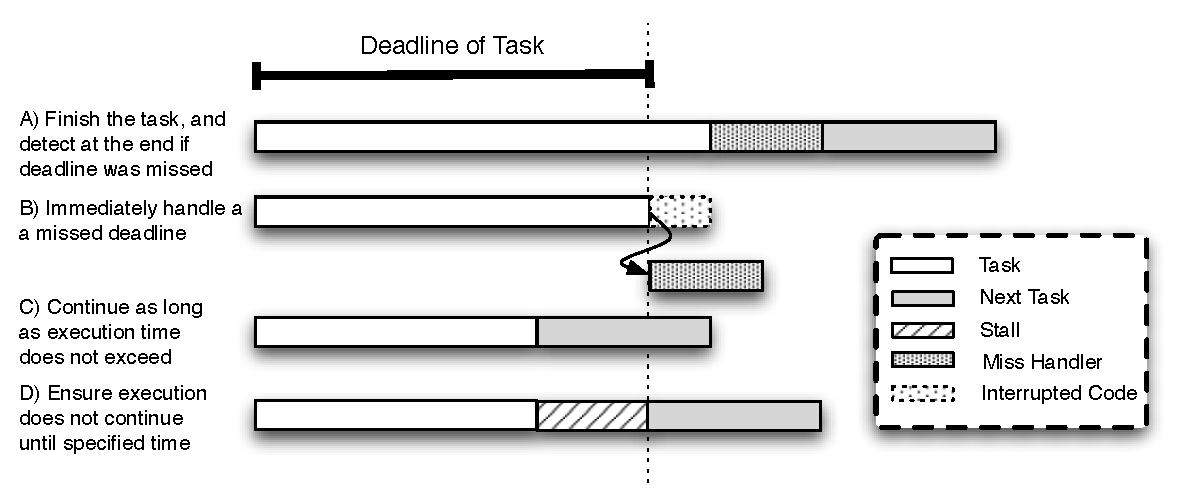
\includegraphics[scale=.7]{figs/timing_behaviors.pdf}
  \end{center}
  \vspace{-3mm}
  \caption{Different Desired Timing Behaviors}
  \label{fig:timing_behaviors}
\end{figure}

If the actual execution time of the task is longer than the specified deadline, the deadline is missed. 
Two possible timing behaviors can be used to handle this situation, which we show in scenario A and B in figure~\ref{fig:timing_behaviors}. 
Scenario A is used if the execution of task needs to completed. 
It could be that the task modifies external I/O states which cannot afford to be left in an unknown state.
In this case, the task is first completed, then a miss handler is executed, and then the next task continues execution.
This is also known as a \emph{late miss detection}.  
Listing~\ref{lst:timing_behavior_A} shows how this is implemented using our timing instructions.
Lines 1 to 3 of the listing is used to setup the deadline timestamp, which is stored in r2 and r3.  
Line 5 branches to the task and returns when the task completes.
Lines 7 to 10 is where the miss detection occurs. 
We simply use another \gettime\ instruction to obtain the current platform time and compare it with the deadline timestamp.
The \emph{blmi} instruction is a \emph{branch with link} instruction that is conditionally executed only if the \emph{[N]egative} condition code is set.
Thus, the branch to \emph{miss\_handler} is only executed if the deadline timestamp is less than the current platform time, which means the deadline was missed.

\begin{lstlisting}[float=h, label=lst:timing_behavior_A,caption=Assembly code to implement scenario A]
  cdp p13, 8, c2, c0, c0, 0  ; get_time, current timestamp stored in [c2, c3]
  adds r3, r3, #0xDEAD       ; assuming the deadline is #0xDEAD
  adc r2, r2, #0             ; lines 2 and 3 calculate the deadline timestamp
   
  bl task                    ; execute Task
  
  cdp p13, 8, c4, c0, c0, 0  ; get_time, current timestamp stored in [c4, c5]
  subs r3, r3, r5            ; lines 8 and 9 check for deadline miss
  sbc  r2, r2, r4            ; 
  blmi miss_handler          ; branch to miss_handler if negative 
                             ; condition code is set
     
  bl task2                   ; execute next task
\end{lstlisting}

If the missed deadline is to be handled immediate, then we cannot check the deadline timestamp in software, but it must be checked in hardware.  
The \exceptiononexpire\ and \deactivateexception\ instructions are then used to immediately execute the \emph{miss\_handler} when the timer expires.
This is shown as scenario B in figure~\ref{fig:timing_behaviors}.
Listing~\ref{lst:timing_behavior_BC} shows the usage of \exceptiononexpire\ and \deactivateexception\ to achieve this timing behavior.
The code is similar the one showed in listing~\ref{lst:exception-sample} for the example usage of \exceptiononexpire\ and \deactivateexception.
In this case, if the \deactivateexception\ is not executed before platform time exceeds the deadline timestamp, then the deadline is missed and the timer expired exception is thrown in hardware.
In the listing we assume that \emph{miss\_handler} has been registered as the exception handler, and will be executed when the timer expired exception is thrown.
The \emph{miss\_handler} can directly abort the finishing of task 1 and directly start task 2, or it could return to the program point where the exception was thrown and continue execution after the \emph{miss\_handler}. 
This is application dependent, and both can be supported in software.   

\begin{lstlisting}[float=h, label=lst:timing_behavior_BC,caption=Assembly code to implement scenario B and C]
  cdp p13, 8, c2, c0, c0, 0  ; get_time, current timestamp stored in [c2, c3]
  adds r3, r3, #0xDEAD       ; assuming the deadline is #0xDEAD
  adc r2, r2, #0             ; lines 2 and 3 calculate the deadline timestamp
  cdp p13, 2, c2, c2, c3, 0  ; exception_on_expire, register [c2, c3]
   
  bl task                    ; execute Task
  
  cdp p13, 5, c0, c0, c0, 0  ; deactivate_exception
     
  bl task2                   ; execute next task
\end{lstlisting}

When the execution time of the task does not exceed the specified deadline, two different behaviors can also be implemented.
The first is shown in scenario C of figure~\ref{fig:timing_behaviors}, where the next task immediately begins to execute.
In this scenario, we merely want to ensure that the task does not exceed the deadline. 
The code shown in the previous listing~\ref{lst:timing_behavior_BC} exhibits this behavior. 
Once the task finishes earlier, \deactivateexception\ is executed to deactivate the exception, and the next task is immediately executed.

However, if we do not want the next task to start until after the specified deadline, then a \delayuntil\ can be used to ensure a minimum execution time for the task.
This could be useful if the tasks are synchronized to an external source.   
The sample code is shown in listing~\ref{lst:timing_behavior_D}, which is scenario D in figure~\ref{fig:timing_behaviors}.

\begin{lstlisting}[float=h, label=lst:timing_behavior_D,caption=Assembly code to implement scenario D]
  cdp p13, 8, c2, c0, c0, 0  ; get_time, current timestamp stored in [c2, c3]
  adds r3, r3, #0xDEAD       ; assuming the deadline is #0xDEAD
  adc r2, r2, #0             ; lines 2 and 3 calculate the deadline timestamp
  cdp p13, 2, c2, c2, c3, 0  ; exception_on_expire, register [c2, c3]
   
  bl task                    ; execute Task
  
  cdp p13, 5, c0, c0, c0, 0  ; deactivate_exception
  cdp p13, 4, c2, c2, c3, 0  ; delay_until 
     
  bl task2                   ; execute next task
\end{lstlisting}

The \delayuntil\ instruction is added after \deactivateexception, and whenever the execution time of the task is less than the specified deadline, it will delay the program until the deadline is reached, ensuring the next task will not execute early.
The order of \delayuntil\ and \deactivateexception\ in this case is very important. 
If the order were the other way around, then \delayuntil\ would first delay the program until after the specified deadline. 
Because \deactivateexception\ has not executed yet, the timer expired exception would always be thrown, even if the task did not miss the deadline.
Thus, \deactivateexception\ must be before \delayuntil.
\Delayuntil\ can also be used in scenario A to achieve the same effect for late miss-detections. 
In that situation, simply insert a \delayuntil\ in line 12 of listing~\ref{lst:timing_behavior_A} and use the first deadline timestamp as its input.    
 
\subsubsection{Timed Loops}
\label{sec:timed_loops}
\begin{figure}
  \vspace{-20pt}
  \begin{center}
    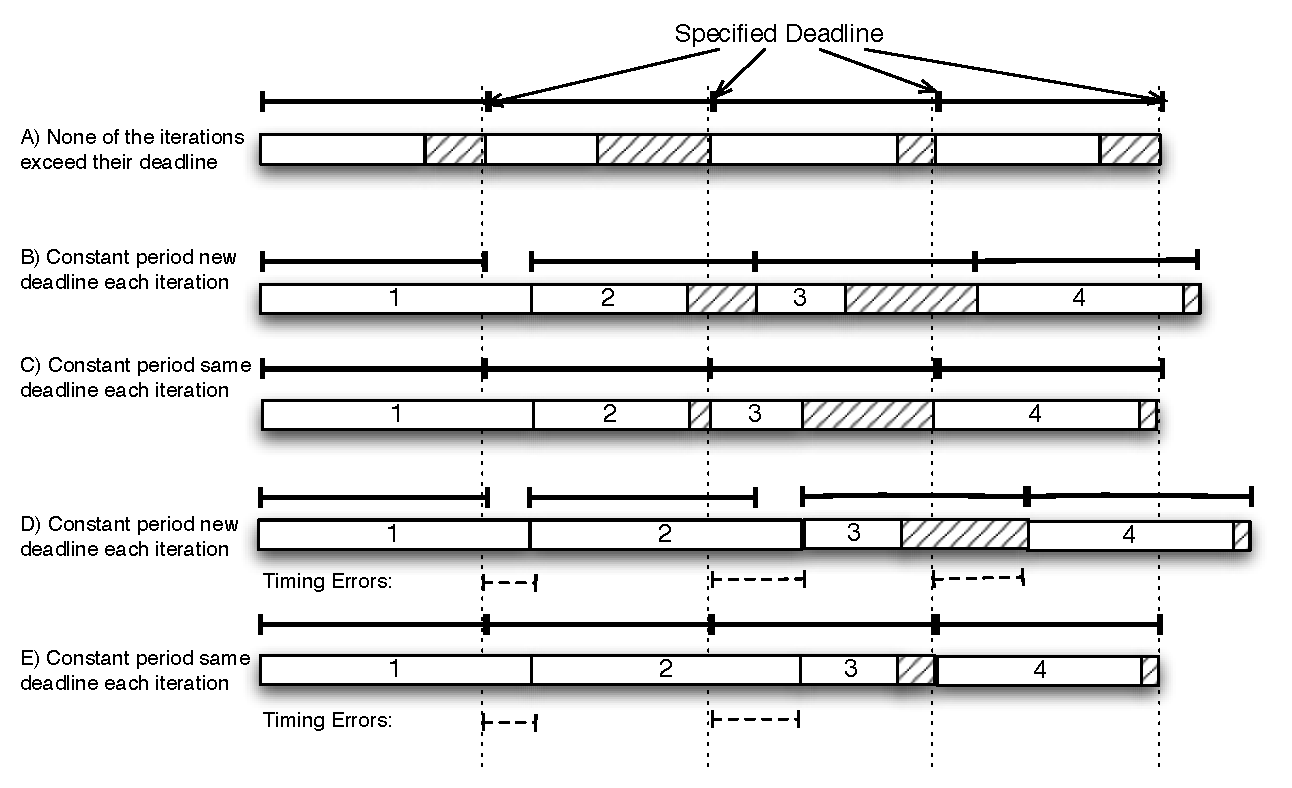
\includegraphics[scale=.7]{figs/timed_loop_differences.pdf}
  \end{center}
  \vspace{-20pt}
  \caption{Timing diagram of different timed loops}
  \label{fig:timed_loop_differences}
\end{figure}
By using timing instructions within loops, we can construct timed loops for programs that exhibit periodic timing behaviors.
Listing~\ref{lst:timed_loop_new_dead} shows sample code that uses \gettime\ and \delayuntil\ to construct a timed loop.

\begin{lstlisting}[float=h, label=lst:timed_loop_new_dead,caption=Timed loops with get\_time and delay\_until ]
loop:
  cdp p13, 8, c2, c0, c0, 0  ; get_time, current timestamp stored in [c2, c3]
  adds r3, r3, #0xDEAD       ; assuming the deadline is #0xDEAD
  adc r2, r2, #0             ; lines 2 and 3 calculate the deadline timestamp
   
  bl task                    ; execute Task
  
  cdp p13, 4, c2, c2, c3, 0  ; delay_until 
  b loop
\end{lstlisting}

The period of each loop iteration is specified by the calculations of line 2 and 3 in listing~\ref{lst:timed_loop_new_dead}, with the small additional time to execute the \gettime\ and \delayuntil\ instruction. 
Ideally, the execution time of the task never exceeds the period of the loop, and the timing behavior shown in scenario A from figure~\ref{fig:timed_loop_differences} is observed. 
In this scenario, each iteration exhibits slightly different execution times, but the \delayuntil\ instruction ensures each iteration takes the whole period to execute.
However, if one iteration misses the deadline its execution time exceeds the period, then scenario B in figure~\ref{fig:timed_loop_differences} would be observed based on our current implementation.
We see that iteration 1 is the only iteration that misses its deadline, but because \gettime\ is called in the beginning of each loop iteration, our next deadline for iteration 2 will be shifted due to the overrun in execution time. 
Even though iteration 2 executes in less time, all future iterations are still shifted after one missed deadline.

The timestamps are stored in general purpose registers and can be manipulated using data-processing instructions, so we can modify slightly the implementation of the timed loop to account for that missed deadline. 
Listing~\ref{lst:timed_loop_same_dead} shows a different implementation of timed loops.
In this implementation, we only call \gettime\ once outside of the loop, and within the loop the deadline timestamps are incremented directly by arithmetic operations, shown on lines 3 and 4.    

\begin{lstlisting}[float=h, label=lst:timed_loop_same_dead,caption=Timed loops with get\_time outside of the loop ]
  cdp p13, 8, c2, c0, c0, 0  ; get_time, current timestamp stored in [c2, c3]
loop:
  adds r3, r3, #0xDEAD       ; assuming the deadline is #0xDEAD
  adc r2, r2, #0             ; lines 3 and 4 calculate the deadline timestamp
   
  bl task                    ; execute Task
  
  cdp p13, 4, c2, c2, c3, 0  ; delay_until 
  b loop
\end{lstlisting}

Figure~\ref{fig:timed_loop_differences} scenario C shows the effects of this implementation. 
Although iteration 1 misses its deadline, but the execution time of iteration 2 is short enough to ``make up'' the delayed time cause from the first iteration.
Future iterations are not effected by the missed deadline from iteration 1, and continue to execute as desired.
By placing \gettime\ outside of the loop, the increments to the deadline timestamp is purely the period of the loop, since we do not call \gettime\ again obtain the current time.
Of course, both implementations are susceptible to the effects of multiple missed deadlines in a row, as shown in scenario D and E.
In this case, both iterations 1 and 2 overrun their deadline, and the timing error is compounded.
With our first implementation of timed loops, the error jitter continues to increase, because the new deadline is set according to the late execution of each iteration, as shown in scenario D. 
The error jitter never recovers, even though iteration 3's execution time is short enough to allow recovery. 
As shown in scenario E, our second iteration recovers the period on the 3rd iteration, and the 4th iteration is not effected. 

Furthermore, we can construct a timed loop that self compensates whenever it detects that an iteration overran its deadline. 
We do so by using the late miss detection mechanism shown previously in our timed loop to run a shorter version of the task whenever a previous deadline is missed.
This is shown in listing~\ref{lst:timed_loop_compensate}. 
\begin{lstlisting}[float=h, label=lst:timed_loop_compensate,caption=Timed loops with compensation ]
  cdp p13, 8, c2, c0, c0, 0  ; get_time, deadline timestamp stored in [c2, c3]
loop:
  cdp p13, 8, c4, c0, c0, 0  ; get_time, current timestamp stored in [c4, c5]
  subs r5, r5, #<offset>     ; <offset> is implementation dependent and used to 
  sbc  r4, r4, #0            ; account for loop overhead and miss detection

  subs r3, r3, r5            ; Check if previous iteration deadline is missed
  sbc  r2, r2, r4            ; 

  blmi task_short            ; execute shorter task if previous deadline mess 
  blpl task_normal           ; or else execute normal task 
  
  adds r3, r3, #0xDEAD       ; assuming the deadline is #0xDEAD
  adc r2, r2, #0             ; calculate the deadline timestamp for this iter.
  cdp p13, 4, c2, c2, c3, 0  ; delay_until
   
  b loop
\end{lstlisting}

In this sample code, we place the late miss detection in the beginning of each loop, and use it to detect if the current platform time is greater than the previously set deadline timestamp.
On lines 4 and 5 we subtract an offset that is used to compensate for the execution time of the loop overhead and miss detection. 
This is an important step that cannot be omitted.
For each iteration, if the previous iteration meets its deadline, the \delayuntil\ instruction will delay program execution until the current platform time exceeds the specified deadline. 
Thus, if the time it takes to execute the loop overhead and miss-detection is not accounted for, then we will always detect a missed deadline from the effects of \delayuntil.  
The actual offset is implementation dependent, depending on how long each instruction takes to execute.
We will show how this offset is calculated in our implementation in section~\ref{sec:timed_loop_revisited}.
Once the overhead is accounted for, lines 7 and 8 check if the previous deadline was met, and lines 10 and 11 executes the short task if the deadline was missed, or executes the normal task else wise.
In this case, we delay the deadline calculation for this iteration until right before the \delayuntil\ instruction, because the miss detection checks against the previous deadline timestamp.      
The timing behavior that is created is shown in figure~\ref{fig:timed_loop_differences} scenario F. 



Other combinations of timing instructions can further be explored.
For example, the use of \exceptiononexpire\ and \deactivateexception\ to handle cases where loop iterations exceeds the period.
In these examples, we are not claiming that a particular implementation of timed loops is the ``correct'' implementation.
We mainly show different possible ways to implement a timed loop construct with our timing extensions, and point out some subtleties when doing so.



